% Created by tikzDevice version 0.12
% !TEX encoding = UTF-8 Unicode
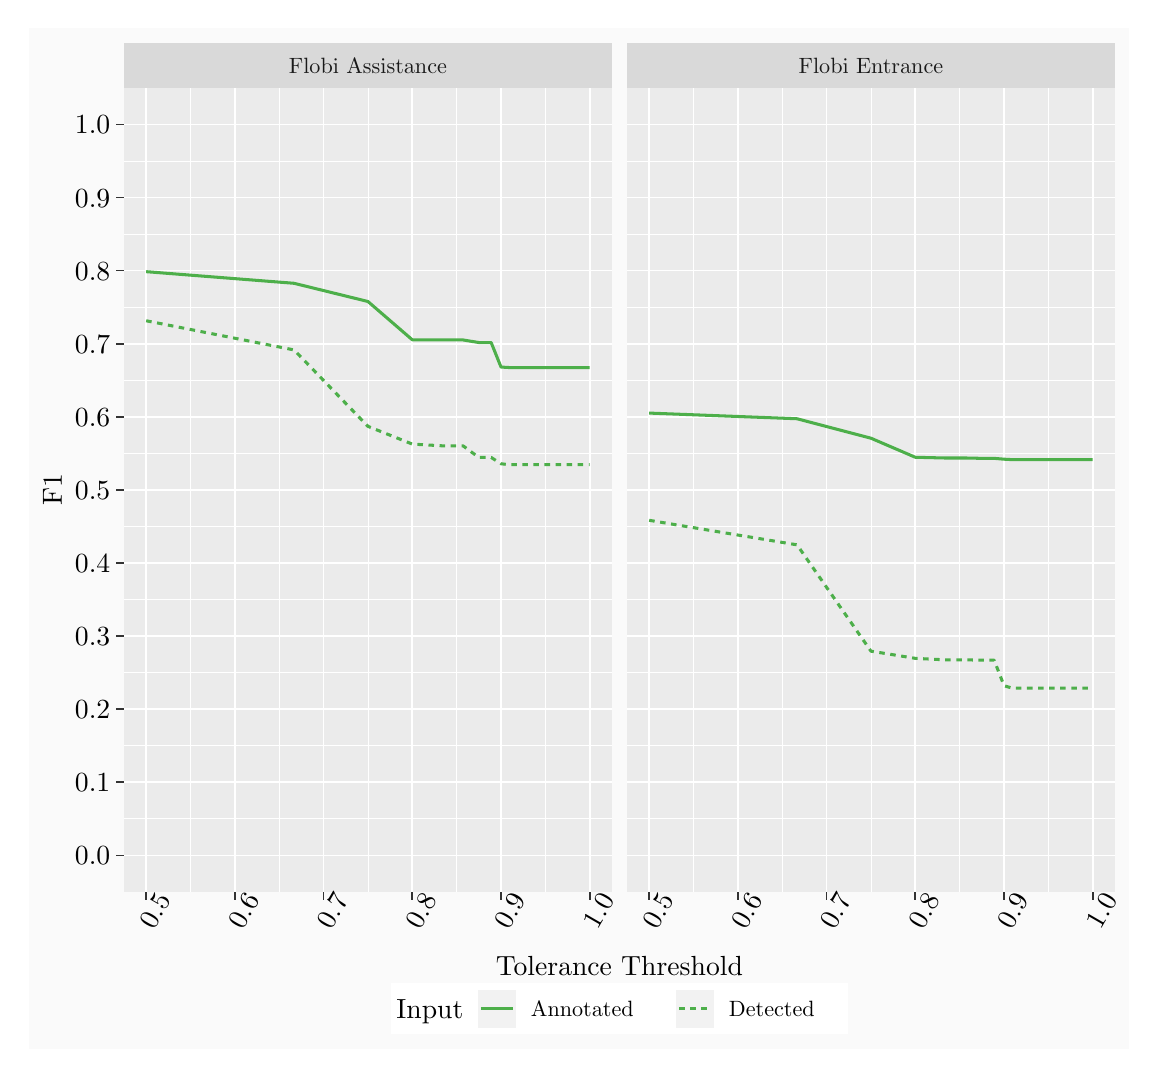
\begin{tikzpicture}[x=1pt,y=1pt]
\definecolor{fillColor}{RGB}{255,255,255}
\path[use as bounding box,fill=fillColor,fill opacity=0.00] (0,0) rectangle (398.34,369.26);
\begin{scope}
\path[clip] (  0.00,  0.00) rectangle (398.34,369.26);
\definecolor{drawColor}{RGB}{255,255,255}
\definecolor{fillColor}{gray}{0.98}

\path[draw=drawColor,line width= 0.6pt,line join=round,line cap=round,fill=fillColor] (  0.00,  0.00) rectangle (398.34,369.26);
\end{scope}
\begin{scope}
\path[clip] ( 34.81, 56.96) rectangle (211.07,347.51);
\definecolor{fillColor}{gray}{0.92}

\path[fill=fillColor] ( 34.81, 56.96) rectangle (211.07,347.51);
\definecolor{drawColor}{RGB}{255,255,255}

\path[draw=drawColor,line width= 0.3pt,line join=round] ( 34.81, 83.38) --
	(211.07, 83.38);

\path[draw=drawColor,line width= 0.3pt,line join=round] ( 34.81,109.79) --
	(211.07,109.79);

\path[draw=drawColor,line width= 0.3pt,line join=round] ( 34.81,136.20) --
	(211.07,136.20);

\path[draw=drawColor,line width= 0.3pt,line join=round] ( 34.81,162.62) --
	(211.07,162.62);

\path[draw=drawColor,line width= 0.3pt,line join=round] ( 34.81,189.03) --
	(211.07,189.03);

\path[draw=drawColor,line width= 0.3pt,line join=round] ( 34.81,215.44) --
	(211.07,215.44);

\path[draw=drawColor,line width= 0.3pt,line join=round] ( 34.81,241.85) --
	(211.07,241.85);

\path[draw=drawColor,line width= 0.3pt,line join=round] ( 34.81,268.27) --
	(211.07,268.27);

\path[draw=drawColor,line width= 0.3pt,line join=round] ( 34.81,294.68) --
	(211.07,294.68);

\path[draw=drawColor,line width= 0.3pt,line join=round] ( 34.81,321.09) --
	(211.07,321.09);

\path[draw=drawColor,line width= 0.3pt,line join=round] ( 58.85, 56.96) --
	( 58.85,347.51);

\path[draw=drawColor,line width= 0.3pt,line join=round] ( 74.87, 56.96) --
	( 74.87,347.51);

\path[draw=drawColor,line width= 0.3pt,line join=round] ( 90.90, 56.96) --
	( 90.90,347.51);

\path[draw=drawColor,line width= 0.3pt,line join=round] (106.93, 56.96) --
	(106.93,347.51);

\path[draw=drawColor,line width= 0.3pt,line join=round] (122.96, 56.96) --
	(122.96,347.51);

\path[draw=drawColor,line width= 0.3pt,line join=round] (155.01, 56.96) --
	(155.01,347.51);

\path[draw=drawColor,line width= 0.3pt,line join=round] (187.06, 56.96) --
	(187.06,347.51);

\path[draw=drawColor,line width= 0.6pt,line join=round] ( 34.81, 70.17) --
	(211.07, 70.17);

\path[draw=drawColor,line width= 0.6pt,line join=round] ( 34.81, 96.58) --
	(211.07, 96.58);

\path[draw=drawColor,line width= 0.6pt,line join=round] ( 34.81,123.00) --
	(211.07,123.00);

\path[draw=drawColor,line width= 0.6pt,line join=round] ( 34.81,149.41) --
	(211.07,149.41);

\path[draw=drawColor,line width= 0.6pt,line join=round] ( 34.81,175.82) --
	(211.07,175.82);

\path[draw=drawColor,line width= 0.6pt,line join=round] ( 34.81,202.24) --
	(211.07,202.24);

\path[draw=drawColor,line width= 0.6pt,line join=round] ( 34.81,228.65) --
	(211.07,228.65);

\path[draw=drawColor,line width= 0.6pt,line join=round] ( 34.81,255.06) --
	(211.07,255.06);

\path[draw=drawColor,line width= 0.6pt,line join=round] ( 34.81,281.47) --
	(211.07,281.47);

\path[draw=drawColor,line width= 0.6pt,line join=round] ( 34.81,307.89) --
	(211.07,307.89);

\path[draw=drawColor,line width= 0.6pt,line join=round] ( 34.81,334.30) --
	(211.07,334.30);

\path[draw=drawColor,line width= 0.6pt,line join=round] ( 42.82, 56.96) --
	( 42.82,347.51);

\path[draw=drawColor,line width= 0.6pt,line join=round] ( 74.87, 56.96) --
	( 74.87,347.51);

\path[draw=drawColor,line width= 0.6pt,line join=round] (106.93, 56.96) --
	(106.93,347.51);

\path[draw=drawColor,line width= 0.6pt,line join=round] (138.98, 56.96) --
	(138.98,347.51);

\path[draw=drawColor,line width= 0.6pt,line join=round] (171.04, 56.96) --
	(171.04,347.51);

\path[draw=drawColor,line width= 0.6pt,line join=round] (203.09, 56.96) --
	(203.09,347.51);
\definecolor{drawColor}{RGB}{77,175,74}

\path[draw=drawColor,line width= 1.1pt,line join=round] ( 42.82,281.09) --
	( 96.24,276.89) --
	(122.96,270.31) --
	(138.98,256.47) --
	(149.67,256.42) --
	(157.30,256.42) --
	(163.02,255.48) --
	(167.48,255.48) --
	(171.04,246.62) --
	(173.95,246.45) --
	(176.38,246.45) --
	(203.06,246.45);

\path[draw=drawColor,line width= 1.1pt,dash pattern=on 2pt off 2pt ,line join=round] ( 42.82,263.35) --
	( 96.24,252.82) --
	(122.96,225.19) --
	(138.98,218.78) --
	(149.67,218.17) --
	(157.30,218.17) --
	(163.02,213.96) --
	(167.48,213.96) --
	(171.04,211.68) --
	(173.95,211.33) --
	(176.38,211.33) --
	(203.06,211.33);
\end{scope}
\begin{scope}
\path[clip] (216.57, 56.96) rectangle (392.84,347.51);
\definecolor{fillColor}{gray}{0.92}

\path[fill=fillColor] (216.57, 56.96) rectangle (392.84,347.51);
\definecolor{drawColor}{RGB}{255,255,255}

\path[draw=drawColor,line width= 0.3pt,line join=round] (216.57, 83.38) --
	(392.84, 83.38);

\path[draw=drawColor,line width= 0.3pt,line join=round] (216.57,109.79) --
	(392.84,109.79);

\path[draw=drawColor,line width= 0.3pt,line join=round] (216.57,136.20) --
	(392.84,136.20);

\path[draw=drawColor,line width= 0.3pt,line join=round] (216.57,162.62) --
	(392.84,162.62);

\path[draw=drawColor,line width= 0.3pt,line join=round] (216.57,189.03) --
	(392.84,189.03);

\path[draw=drawColor,line width= 0.3pt,line join=round] (216.57,215.44) --
	(392.84,215.44);

\path[draw=drawColor,line width= 0.3pt,line join=round] (216.57,241.85) --
	(392.84,241.85);

\path[draw=drawColor,line width= 0.3pt,line join=round] (216.57,268.27) --
	(392.84,268.27);

\path[draw=drawColor,line width= 0.3pt,line join=round] (216.57,294.68) --
	(392.84,294.68);

\path[draw=drawColor,line width= 0.3pt,line join=round] (216.57,321.09) --
	(392.84,321.09);

\path[draw=drawColor,line width= 0.3pt,line join=round] (240.61, 56.96) --
	(240.61,347.51);

\path[draw=drawColor,line width= 0.3pt,line join=round] (256.64, 56.96) --
	(256.64,347.51);

\path[draw=drawColor,line width= 0.3pt,line join=round] (272.67, 56.96) --
	(272.67,347.51);

\path[draw=drawColor,line width= 0.3pt,line join=round] (288.69, 56.96) --
	(288.69,347.51);

\path[draw=drawColor,line width= 0.3pt,line join=round] (304.72, 56.96) --
	(304.72,347.51);

\path[draw=drawColor,line width= 0.3pt,line join=round] (336.78, 56.96) --
	(336.78,347.51);

\path[draw=drawColor,line width= 0.3pt,line join=round] (368.83, 56.96) --
	(368.83,347.51);

\path[draw=drawColor,line width= 0.6pt,line join=round] (216.57, 70.17) --
	(392.84, 70.17);

\path[draw=drawColor,line width= 0.6pt,line join=round] (216.57, 96.58) --
	(392.84, 96.58);

\path[draw=drawColor,line width= 0.6pt,line join=round] (216.57,123.00) --
	(392.84,123.00);

\path[draw=drawColor,line width= 0.6pt,line join=round] (216.57,149.41) --
	(392.84,149.41);

\path[draw=drawColor,line width= 0.6pt,line join=round] (216.57,175.82) --
	(392.84,175.82);

\path[draw=drawColor,line width= 0.6pt,line join=round] (216.57,202.24) --
	(392.84,202.24);

\path[draw=drawColor,line width= 0.6pt,line join=round] (216.57,228.65) --
	(392.84,228.65);

\path[draw=drawColor,line width= 0.6pt,line join=round] (216.57,255.06) --
	(392.84,255.06);

\path[draw=drawColor,line width= 0.6pt,line join=round] (216.57,281.47) --
	(392.84,281.47);

\path[draw=drawColor,line width= 0.6pt,line join=round] (216.57,307.89) --
	(392.84,307.89);

\path[draw=drawColor,line width= 0.6pt,line join=round] (216.57,334.30) --
	(392.84,334.30);

\path[draw=drawColor,line width= 0.6pt,line join=round] (224.58, 56.96) --
	(224.58,347.51);

\path[draw=drawColor,line width= 0.6pt,line join=round] (256.64, 56.96) --
	(256.64,347.51);

\path[draw=drawColor,line width= 0.6pt,line join=round] (288.69, 56.96) --
	(288.69,347.51);

\path[draw=drawColor,line width= 0.6pt,line join=round] (320.75, 56.96) --
	(320.75,347.51);

\path[draw=drawColor,line width= 0.6pt,line join=round] (352.80, 56.96) --
	(352.80,347.51);

\path[draw=drawColor,line width= 0.6pt,line join=round] (384.86, 56.96) --
	(384.86,347.51);
\definecolor{drawColor}{RGB}{77,175,74}

\path[draw=drawColor,line width= 1.1pt,line join=round] (224.58,229.99) --
	(278.01,227.94) --
	(304.72,220.91) --
	(320.75,214.02) --
	(331.43,213.76) --
	(339.07,213.76) --
	(344.79,213.63) --
	(349.24,213.63) --
	(352.80,213.33) --
	(355.72,213.17) --
	(358.15,213.17) --
	(384.83,213.17);

\path[draw=drawColor,line width= 1.1pt,dash pattern=on 2pt off 2pt ,line join=round] (224.58,191.24) --
	(278.01,182.38) --
	(304.72,143.96) --
	(320.75,141.36) --
	(331.43,140.83) --
	(339.07,140.83) --
	(344.79,140.69) --
	(349.24,140.69) --
	(352.80,131.47) --
	(355.72,130.62) --
	(358.15,130.62) --
	(384.83,130.62);
\end{scope}
\begin{scope}
\path[clip] ( 34.81,347.51) rectangle (211.07,363.76);
\definecolor{fillColor}{gray}{0.85}

\path[fill=fillColor] ( 34.81,347.51) rectangle (211.07,363.76);
\definecolor{drawColor}{gray}{0.10}

\node[text=drawColor,anchor=base,inner sep=0pt, outer sep=0pt, scale=  0.80] at (122.94,352.88) {Flobi Assistance};
\end{scope}
\begin{scope}
\path[clip] (216.57,347.51) rectangle (392.84,363.76);
\definecolor{fillColor}{gray}{0.85}

\path[fill=fillColor] (216.57,347.51) rectangle (392.84,363.76);
\definecolor{drawColor}{gray}{0.10}

\node[text=drawColor,anchor=base,inner sep=0pt, outer sep=0pt, scale=  0.80] at (304.71,352.88) {Flobi Entrance};
\end{scope}
\begin{scope}
\path[clip] (  0.00,  0.00) rectangle (398.34,369.26);
\definecolor{drawColor}{gray}{0.20}

\path[draw=drawColor,line width= 0.6pt,line join=round] ( 42.82, 54.21) --
	( 42.82, 56.96);

\path[draw=drawColor,line width= 0.6pt,line join=round] ( 74.87, 54.21) --
	( 74.87, 56.96);

\path[draw=drawColor,line width= 0.6pt,line join=round] (106.93, 54.21) --
	(106.93, 56.96);

\path[draw=drawColor,line width= 0.6pt,line join=round] (138.98, 54.21) --
	(138.98, 56.96);

\path[draw=drawColor,line width= 0.6pt,line join=round] (171.04, 54.21) --
	(171.04, 56.96);

\path[draw=drawColor,line width= 0.6pt,line join=round] (203.09, 54.21) --
	(203.09, 56.96);
\end{scope}
\begin{scope}
\path[clip] (  0.00,  0.00) rectangle (398.34,369.26);
\definecolor{drawColor}{RGB}{0,0,0}

\node[text=drawColor,rotate= 60.00,anchor=base,inner sep=0pt, outer sep=0pt, scale=  1.00] at ( 48.78, 48.57) {0.5};

\node[text=drawColor,rotate= 60.00,anchor=base,inner sep=0pt, outer sep=0pt, scale=  1.00] at ( 80.84, 48.57) {0.6};

\node[text=drawColor,rotate= 60.00,anchor=base,inner sep=0pt, outer sep=0pt, scale=  1.00] at (112.89, 48.57) {0.7};

\node[text=drawColor,rotate= 60.00,anchor=base,inner sep=0pt, outer sep=0pt, scale=  1.00] at (144.95, 48.57) {0.8};

\node[text=drawColor,rotate= 60.00,anchor=base,inner sep=0pt, outer sep=0pt, scale=  1.00] at (177.00, 48.57) {0.9};

\node[text=drawColor,rotate= 60.00,anchor=base,inner sep=0pt, outer sep=0pt, scale=  1.00] at (209.06, 48.57) {1.0};
\end{scope}
\begin{scope}
\path[clip] (  0.00,  0.00) rectangle (398.34,369.26);
\definecolor{drawColor}{gray}{0.20}

\path[draw=drawColor,line width= 0.6pt,line join=round] (224.58, 54.21) --
	(224.58, 56.96);

\path[draw=drawColor,line width= 0.6pt,line join=round] (256.64, 54.21) --
	(256.64, 56.96);

\path[draw=drawColor,line width= 0.6pt,line join=round] (288.69, 54.21) --
	(288.69, 56.96);

\path[draw=drawColor,line width= 0.6pt,line join=round] (320.75, 54.21) --
	(320.75, 56.96);

\path[draw=drawColor,line width= 0.6pt,line join=round] (352.80, 54.21) --
	(352.80, 56.96);

\path[draw=drawColor,line width= 0.6pt,line join=round] (384.86, 54.21) --
	(384.86, 56.96);
\end{scope}
\begin{scope}
\path[clip] (  0.00,  0.00) rectangle (398.34,369.26);
\definecolor{drawColor}{RGB}{0,0,0}

\node[text=drawColor,rotate= 60.00,anchor=base,inner sep=0pt, outer sep=0pt, scale=  1.00] at (230.55, 48.57) {0.5};

\node[text=drawColor,rotate= 60.00,anchor=base,inner sep=0pt, outer sep=0pt, scale=  1.00] at (262.60, 48.57) {0.6};

\node[text=drawColor,rotate= 60.00,anchor=base,inner sep=0pt, outer sep=0pt, scale=  1.00] at (294.66, 48.57) {0.7};

\node[text=drawColor,rotate= 60.00,anchor=base,inner sep=0pt, outer sep=0pt, scale=  1.00] at (326.71, 48.57) {0.8};

\node[text=drawColor,rotate= 60.00,anchor=base,inner sep=0pt, outer sep=0pt, scale=  1.00] at (358.77, 48.57) {0.9};

\node[text=drawColor,rotate= 60.00,anchor=base,inner sep=0pt, outer sep=0pt, scale=  1.00] at (390.82, 48.57) {1.0};
\end{scope}
\begin{scope}
\path[clip] (  0.00,  0.00) rectangle (398.34,369.26);
\definecolor{drawColor}{RGB}{0,0,0}

\node[text=drawColor,anchor=base east,inner sep=0pt, outer sep=0pt, scale=  1.00] at ( 29.86, 66.73) {0.0};

\node[text=drawColor,anchor=base east,inner sep=0pt, outer sep=0pt, scale=  1.00] at ( 29.86, 93.14) {0.1};

\node[text=drawColor,anchor=base east,inner sep=0pt, outer sep=0pt, scale=  1.00] at ( 29.86,119.55) {0.2};

\node[text=drawColor,anchor=base east,inner sep=0pt, outer sep=0pt, scale=  1.00] at ( 29.86,145.97) {0.3};

\node[text=drawColor,anchor=base east,inner sep=0pt, outer sep=0pt, scale=  1.00] at ( 29.86,172.38) {0.4};

\node[text=drawColor,anchor=base east,inner sep=0pt, outer sep=0pt, scale=  1.00] at ( 29.86,198.79) {0.5};

\node[text=drawColor,anchor=base east,inner sep=0pt, outer sep=0pt, scale=  1.00] at ( 29.86,225.20) {0.6};

\node[text=drawColor,anchor=base east,inner sep=0pt, outer sep=0pt, scale=  1.00] at ( 29.86,251.62) {0.7};

\node[text=drawColor,anchor=base east,inner sep=0pt, outer sep=0pt, scale=  1.00] at ( 29.86,278.03) {0.8};

\node[text=drawColor,anchor=base east,inner sep=0pt, outer sep=0pt, scale=  1.00] at ( 29.86,304.44) {0.9};

\node[text=drawColor,anchor=base east,inner sep=0pt, outer sep=0pt, scale=  1.00] at ( 29.86,330.86) {1.0};
\end{scope}
\begin{scope}
\path[clip] (  0.00,  0.00) rectangle (398.34,369.26);
\definecolor{drawColor}{gray}{0.20}

\path[draw=drawColor,line width= 0.6pt,line join=round] ( 32.06, 70.17) --
	( 34.81, 70.17);

\path[draw=drawColor,line width= 0.6pt,line join=round] ( 32.06, 96.58) --
	( 34.81, 96.58);

\path[draw=drawColor,line width= 0.6pt,line join=round] ( 32.06,123.00) --
	( 34.81,123.00);

\path[draw=drawColor,line width= 0.6pt,line join=round] ( 32.06,149.41) --
	( 34.81,149.41);

\path[draw=drawColor,line width= 0.6pt,line join=round] ( 32.06,175.82) --
	( 34.81,175.82);

\path[draw=drawColor,line width= 0.6pt,line join=round] ( 32.06,202.24) --
	( 34.81,202.24);

\path[draw=drawColor,line width= 0.6pt,line join=round] ( 32.06,228.65) --
	( 34.81,228.65);

\path[draw=drawColor,line width= 0.6pt,line join=round] ( 32.06,255.06) --
	( 34.81,255.06);

\path[draw=drawColor,line width= 0.6pt,line join=round] ( 32.06,281.47) --
	( 34.81,281.47);

\path[draw=drawColor,line width= 0.6pt,line join=round] ( 32.06,307.89) --
	( 34.81,307.89);

\path[draw=drawColor,line width= 0.6pt,line join=round] ( 32.06,334.30) --
	( 34.81,334.30);
\end{scope}
\begin{scope}
\path[clip] (  0.00,  0.00) rectangle (398.34,369.26);
\definecolor{drawColor}{RGB}{0,0,0}

\node[text=drawColor,anchor=base,inner sep=0pt, outer sep=0pt, scale=  1.00] at (213.82, 26.90) {Tolerance Threshold};
\end{scope}
\begin{scope}
\path[clip] (  0.00,  0.00) rectangle (398.34,369.26);
\definecolor{drawColor}{RGB}{0,0,0}

\node[text=drawColor,rotate= 90.00,anchor=base,inner sep=0pt, outer sep=0pt, scale=  1.00] at ( 12.39,202.24) {F1};
\end{scope}
\begin{scope}
\path[clip] (  0.00,  0.00) rectangle (398.34,369.26);
\definecolor{fillColor}{RGB}{255,255,255}

\path[fill=fillColor] (131.24,  5.50) rectangle (296.40, 23.95);
\end{scope}
\begin{scope}
\path[clip] (  0.00,  0.00) rectangle (398.34,369.26);
\definecolor{drawColor}{RGB}{0,0,0}

\node[text=drawColor,anchor=base west,inner sep=0pt, outer sep=0pt, scale=  1.00] at (133.24, 11.28) {Input};
\end{scope}
\begin{scope}
\path[clip] (  0.00,  0.00) rectangle (398.34,369.26);
\definecolor{drawColor}{RGB}{255,255,255}
\definecolor{fillColor}{gray}{0.95}

\path[draw=drawColor,line width= 0.6pt,line join=round,line cap=round,fill=fillColor] (162.40,  7.50) rectangle (176.86, 21.95);
\end{scope}
\begin{scope}
\path[clip] (  0.00,  0.00) rectangle (398.34,369.26);
\definecolor{drawColor}{RGB}{77,175,74}

\path[draw=drawColor,line width= 1.1pt,line join=round] (163.85, 14.73) -- (175.41, 14.73);
\end{scope}
\begin{scope}
\path[clip] (  0.00,  0.00) rectangle (398.34,369.26);
\definecolor{drawColor}{RGB}{255,255,255}
\definecolor{fillColor}{gray}{0.95}

\path[draw=drawColor,line width= 0.6pt,line join=round,line cap=round,fill=fillColor] (233.96,  7.50) rectangle (248.41, 21.95);
\end{scope}
\begin{scope}
\path[clip] (  0.00,  0.00) rectangle (398.34,369.26);
\definecolor{drawColor}{RGB}{77,175,74}

\path[draw=drawColor,line width= 1.1pt,dash pattern=on 2pt off 2pt ,line join=round] (235.40, 14.73) -- (246.97, 14.73);
\end{scope}
\begin{scope}
\path[clip] (  0.00,  0.00) rectangle (398.34,369.26);
\definecolor{drawColor}{RGB}{0,0,0}

\node[text=drawColor,anchor=base west,inner sep=0pt, outer sep=0pt, scale=  0.80] at (181.86, 11.97) {Annotated};
\end{scope}
\begin{scope}
\path[clip] (  0.00,  0.00) rectangle (398.34,369.26);
\definecolor{drawColor}{RGB}{0,0,0}

\node[text=drawColor,anchor=base west,inner sep=0pt, outer sep=0pt, scale=  0.80] at (253.41, 11.97) {Detected};
\end{scope}
\end{tikzpicture}
